\chapter{Fundamentação teórica}
%\section{Revisão bibliográfica}
Neste capítulo analisou-se a bibliografia existe e executou-se uma revisão em trabalhos correlatos. Nela pesquisou-se sobre arquiteturas de rede disponíveis para utilização durante comunicações de dispositivos IoT, bem como técnicas para aproveitamento de energia disponíveis no ambiente.

%%%%%%%%%%%%%%%%%%%%%%%%%%%%%%%%%%%%%%%%%%%%%%%%%%%%%%%%%%%%%%%%%%%%%%
\section{LPWAN} %ch 1303
%%%%%%%%%%%%%%%%%%%%%%%%%%%%%%%%%%%%%%%%%%%%%%%%%%%%%%%%%%%%%%%%%%%%%%
Para dispositivos IoT, um dos objetivos é transmitir dados sem fio usando o mínimo de energia possível. Por isso, os projetistas de aplicações com sensores alimentados por bateria estão particularmente preocupados em enviar dados de sensores de baixa taxa de dados, utilizando comunicação sem fio por quilômetros para minimizar o uso da bateria. Entre as soluções existentes, Bluetooth e Zigbee são projetados para aplicações de curto alcance, já as redes de dados de celular precisam comportar uma quantidade massiva de dados. As \textit{Low-power wide-area network}(LPWAN) que tornaram-se uma solução popular para este problema. Na figura~\ref{fig:LPWAN} é possível ver alguns tipos de redes em função do alcance e largura de rede, com destaque especial para as redes LPWAN.
%\FloatBarrier 
\begin{figure}
  \caption{Tipos de redes em função do alcance e da largura de banda.}
  \begin{center}
      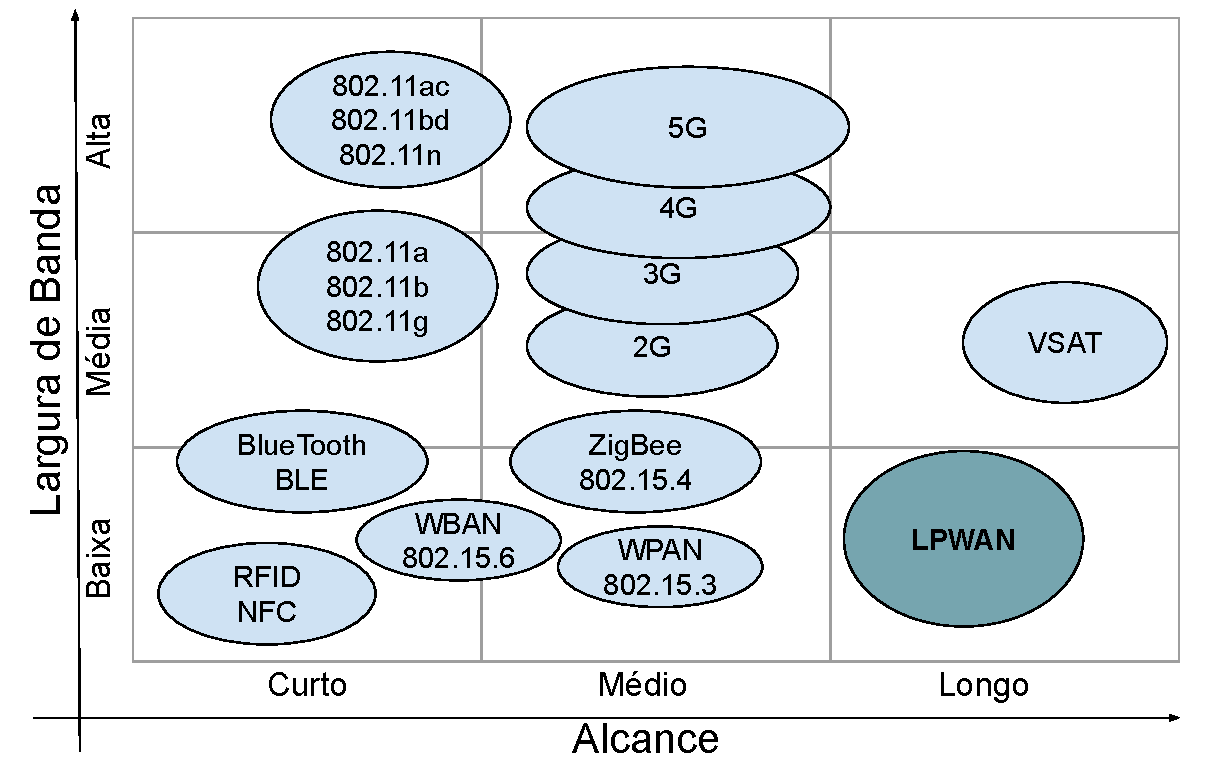
\includegraphics[scale=0.7]{img/LPWAN.pdf}
  \end{center}
  \fonte{Elaborado pelo autor.}
  \label{fig:LPWAN}
\end{figure}
%\FloatBarrier 
Redes \textit{LPWAN} tem crescido em volume devido a sua versatilidade em aplicações \textit{IoT} significativamente desde 2017. De acordo com \citeonline{Mane2021}, as duas principais tecnologias que dominam este mercado, \textit{LoRa} e \textit{Sigfox} apresentam resultados de performance compatíveis para esse tipo de aplicação, podendo ainda possuir configurações diferentes de ganhos para cada necessidade.


%%%%%%%%%%%%%%%%%%%%%%%%%%%%%%%%%%%%%%%%%%%%%%%%%%%%%%%%%%%%%%%%%%%%%%
\subsection{LoRa}
LoRa\cite{LoRaAlliance} é a camada física ou a modulação sem fio utilizada para criar o link de comunicação de longo alcance. Muitos sistemas sem fio legados usam a modulação FSK (Frequency Shifting Keying) como a camada física porque é uma modulação muito eficiente para alcançar baixa potência. O LoRa é baseado na modulação de espalhamento espectral, que mantém as mesmas características de baixa potência da modulação FSK, mas aumenta significativamente o alcance da comunicação. 

Esta comunicação é semelhante ao FM, pois modula um sinal alterando sua frequência. No entanto, enquanto um sinal FM muda a frequência instantaneamente, um sinal LoRa aumenta ou diminui a frequência lentamente ao longo de um período de tempo. Esse aumento ou diminuição gradual é chamado de \textit{chirp}, e a taxa de mudança de frequência ao longo do tempo é chamada de \textit{`chirpiness'}. 

O espalhamento espectral tem sido usado em comunicações militares e espaciais por décadas devido às longas distâncias de comunicação que podem ser alcançadas e robustez à interferência, mas o LoRa é a primeira implementação de baixo custo para uso comercial.

As redes LoRaWAN distribuem-se em uma topologia estrela, com protocolos de comunicação e acesso projetados para usar o mínimo de energia e minimizar colisões de sinal de vários terminais. Cada \textit{endpoint} envia seus dados para um \textit{gateway}, que transmite os dados para outra rede, como Ethernet ou Wi-Fi. Os dados recebidos pelo \textit{gateway} são transmitidos pela rede para um computador central que fará o armazenamento ou processamento adicional.
%%%%%%%%%%%%%%%%%%%%%%%%%%%%%%%%%%%%%%%%%%%%%%%%%%%%%%%%%%%%%%%%%%%%%%
\subsection{Sigfox}
%%%%%%%%%%%%%%%%%%%%%%%%%%%%%%%%%%%%%%%%%%%%%%%%%%%%%%%%%%%%%%%%%%%%%%

Esta abordagem única no mundo da conectividade sem fio, onde não há sobrecarga de sinalização, um protocolo compacto e otimizado e onde o compartilhamento de objetos não está conectado à rede.
A Sigfox oferece uma solução de comunicação baseada em software, onde toda a complexidade de rede e computação é gerenciada na nuvem, e não nos dispositivos. Tudo isso junto, reduz drasticamente o consumo de energia e os custos dos dispositivos conectados.


Um dos desafios mais significativos enfrentados pela Internet das Coisas (IoT) é a capacidade de adicionar nós sensores sem fio de maneira fácil e econômica. Sigfox é uma rede proprietária destinada a ouvir bilhões de objetos transmitindo dados, sem a necessidade de estabelecer e manter conexões de rede. O link sem fio precisa ser de baixa potência para que os nós possam funcionar por anos com uma única bateria e ainda ter longo alcance para que milhares de nós possam se conectar ao gateway para coletar dados.

A empresa francesa Sigfox desenvolveu um protocolo de rádio de baixa potência, implementação de rede e infraestrutura de computação em nuvem que pode ser usado para conectar milhões de dispositivos sem fio de baixa potência. Para isso, o protocolo de baixo consumo combinado com uma rede de \textit{gateways} semelhantes a sistemas de telefonia celular, mas que diferentemente de aplicações \textit{machine-to-machine} (M2M) em redes celulares, as redes Sigfox são dedicadas a dispositivos IoT para monitoramento de saúde, energia, temperatura e umidade e até mesmo sensores de segurança.

A rede foi otimizada para longo alcance e baixa potência usando modulação do tipo \textit{differential binary phase shift keying} (DBPSK). Este é um tipo de modulação robusto e altamente eficiente que transporta um bit por símbolo e não precisa de recuperação de portadora. A robustez da codificação permite o longo alcance, e a simplicidade ajuda a manter o consumo de energia baixo, pois pode ser tratado por um processador de 8 bits. Com uma taxa de dados de 100 bits/s é adequada para aplicações de nó de sensor sem fio de longo alcance e baixa potência com atualizações regulares de pequenas quantidades de dados.


%%%%%%%%%%%%%%%%%%%%%%%%%%%%%%%%%%%%%%%%%%%%%%%%%%%%%%%%%%%%%%%%%%%%%%
\subsection{Escolha do protocolo}
%%%%%%%%%%%%%%%%%%%%%%%%%%%%%%%%%%%%%%%%%%%%%%%%%%%%%%%%%%%%%%%%%%%%%%
Redes LoRaWAN e Sigfox, apresentam soluções que podem divergir sobre alguns aspectos, como o fato das redes LoRaWAN necessitarem de uma implementação da infraestrutura de rede com gateway e servidores. Já na rede Sigfox, a infraestrutura de rede é comercializada pela própria empresa, imputando à solução o pagamento de taxas relacionadas à comunicação. O quadro~\ref{qd:LoraVsSigfox} apresenta uma comparação entra as características técnicas de cada tecnologia.

\begin{quadro}
\caption{Comparação entre LoRa e Sigfox.}
\label{qd:LoraVsSigfox}
  \begin{center}
      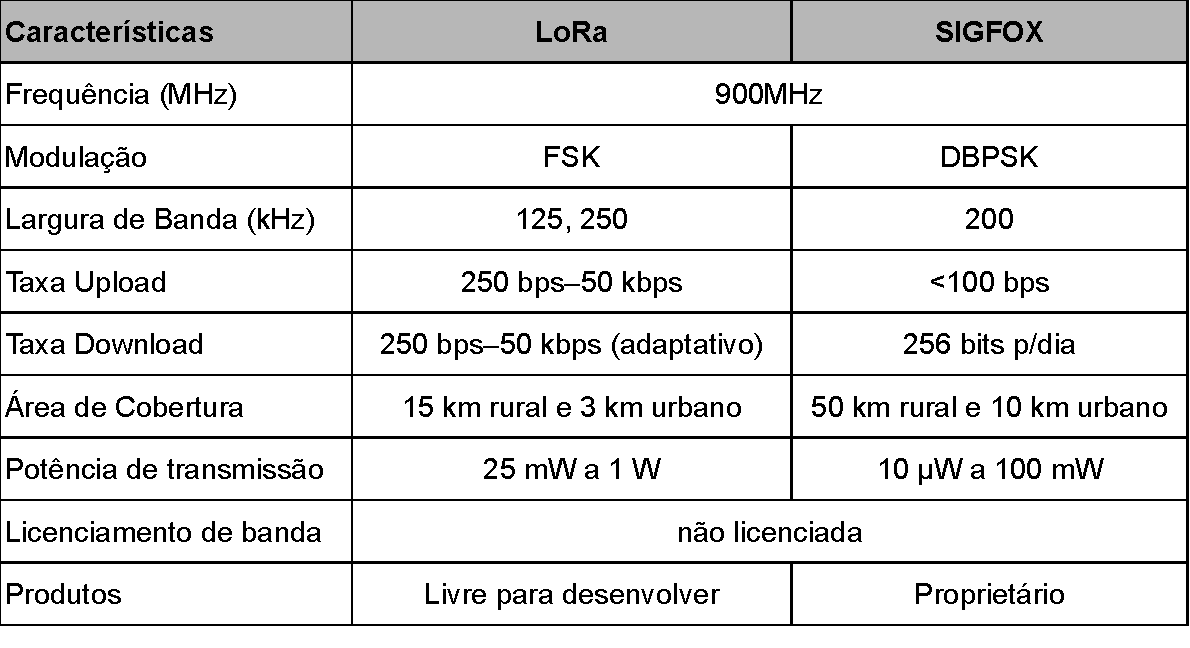
\includegraphics[scale=0.76]{img/LoraVsSigfox.pdf}
  \end{center}
\fonte{Elaborado pelo autor.}
\end{quadro}

No estudo apresentado por \citeonline{Osman2018}, concluiu-se que a tecnologia Sigfox apresenta uma menor taxa de colisões por pacote. Somando-se isso ao fato de existir uma infraestrutura de rede privada para este tipo de aplicação, pode-se dizer que a escolha deste tipo de rede apresenta vantagens.

Entretanto, cabe ressaltar que as duas tecnologias apresentam características suficientes para implementação da solução a que esse trabalho se propõe. Neste trabalho no entanto, optou-se por uso de um recurso de hardware disponibilizado pela empresa HT Micron para fins de estudo capaz de estabelecer uma comunicação do tipo indicado para redes Sigfox.
%%%%%%%%%%%%%%%%%%%%%%%%%%%%%%%%%%%%%%%%%%%%%%%%%%%%%%%%%%%%%%%%%%%%%%
\section{Energy Harvesting}
%%%%%%%%%%%%%%%%%%%%%%%%%%%%%%%%%%%%%%%%%%%%%%%%%%%%%%%%%%%%%%%%%%%%%%
\textit{Energy Harvesting} (EH) é um termo em inglês que pode ser traduzido como ``Captura de Energia'' e consiste e coletar energia de algum meio para empregar em um outro uso. Por milênios os seres humanos vêm criando e aperfeiçoando técnicas de coletar energia de um modo cada vez mais eficiente e diversificado.

As técnicas podem variar, mas pode-se coletar energia atualmente com as seguintes fontes: solar, de vibrações, térmica, cinética, piezoelétrica e de radiofrequência. Muitas fontes de energia se consolidaram no último século como a cinética em casos que transforma o movimento dos rios em energia através de usinas hidrelétrica, bem como os painéis solares que transformam a energia solar e eletricidade. Entretanto, estes meios caracterizam-se por converter grandes volumes de energia para abastecer grandes populações. 

Já em sistemas IoT que necessitam de mobilidade, esta tarefa encontra um dificultador devido ao espaço que estes capturadores de energia necessitam. Além do mais, devido a mobilidade, nem sempre algumas fontes podem estar presente, como a luz solar, uma vez que este sistema se encontre em um local fechado. 

Nestes casos, a escolha da fonte de energia deve ser analisada respeitando os critérios de disponibilidade da fonte nos locais por onde este dispositivo efetuará o seu deslocamento. Dentre as possibilidades de aproveitamento de energia para sistemas IoT, um deles se destaca por sua crescente disponibilidade. O crescente aumento do número de dispositivos de RF para redes ISM(\textit{industrial, scientific and medical}) aponta para um caminho de alta disponibilidade de potência de sinal disponível nesta banda de frequência. No Brasil, a faixa que compreende as frequências de $902MHz$ até $928MHz$ alocou-se para este tipo de aplicações. Em um estudo realizado por~\citeonline{manuel}, pode-se obter uma medição da potência de sinal de RF ao logo de uma faixa do espectro de frequências em uma estação de metrô da Inglaterra. Pode-se observar na figura~\ref{fig:espectro} que nesta mesma faixa citada acima, há uma grande alocação de potência, indicando significativa disponibilidade de energia a ser coletada.

\begin{figure}
  \caption{Densidade de potência de RF medida fora da estação Northfields London.}
  \begin{center}
      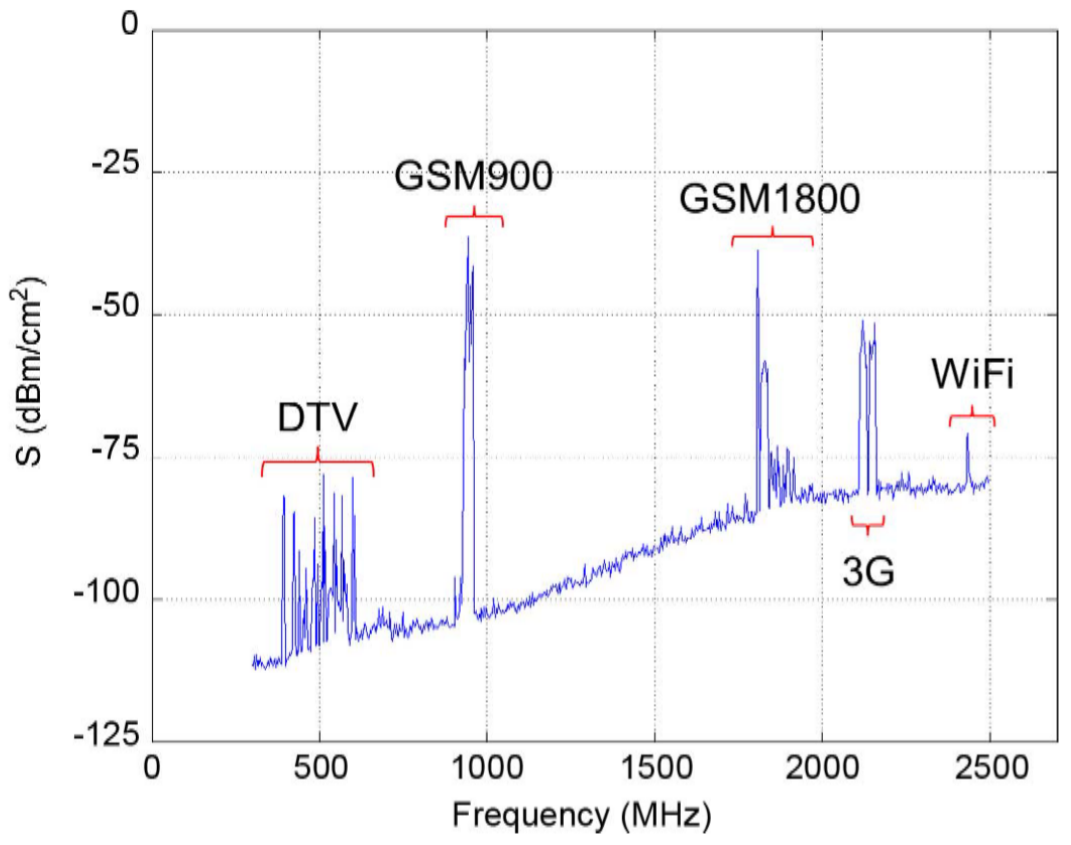
\includegraphics[scale=0.4]{img/espectro.png}
  \end{center}
  \fonte{~\cite{manuel} }
  \label{fig:espectro}
\end{figure}

%%%%%%%%%%%%%%%%%%%%%%%%%%%%%%%%%%%%%%%%%%%%%%%%%%%%%%%%%%%%%%%%%%%%%%


Todos os trabalhos mencionados no quadro~\ref{qd:correlatos} possuem as suas particularidades de aplicação à projetos que envolvem a análise ou monitoramento de redes inteligentes de distribuição de produtos perecíveis. Não necessariamente envolvendo alimentos, ou especificamente o monitoramento, mas traçando algum paralelo com o presente trabalho.
Alguns dos trabalhos são mais superficiais, outros mais profundos, porém todos demonstram alinhamento com o tema proposto.

\begin{quadro}
  \caption{Trabalhos Correlatos.}
  \begin{center}
      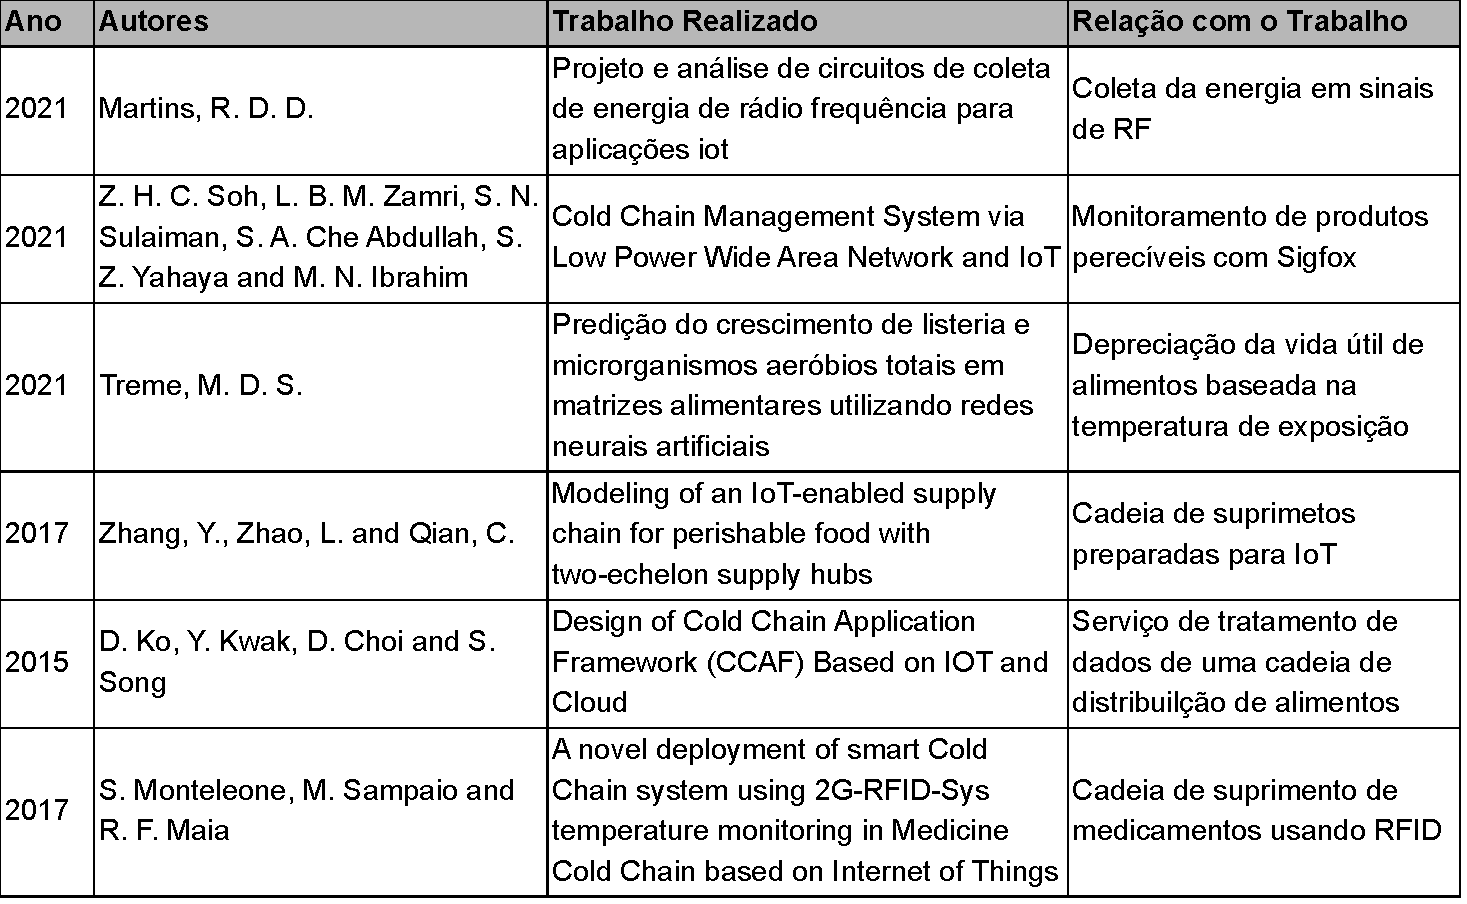
\includegraphics[scale=0.64]{img/correlatos.pdf}
  \end{center}
  \fonte{Elaborado pelo autor.}
  \label{qd:correlatos}
\end{quadro}


%%%%%%%%%%%%%%%%%%%%%%%%%%%%%%%%%%%%%%%%%%%%%%%%%%%%%%%%%%%%%%%%%%%%%%

